%DIF PREAMBLE EXTENSION ADDED BY LATEXDIFF
%DIF UNDERLINE PREAMBLE %DIF PREAMBLE
\RequirePackage[normalem]{ulem} %DIF PREAMBLE
\RequirePackage{color}\definecolor{RED}{rgb}{1,0,0}\definecolor{BLUE}{rgb}{0,0,1} %DIF PREAMBLE
\providecommand{\DIFadd}[1]{{\protect\color{blue}\uwave{#1}}} %DIF PREAMBLE
\providecommand{\DIFdel}[1]{{\protect\color{red}\sout{#1}}}                      %DIF PREAMBLE
%DIF SAFE PREAMBLE %DIF PREAMBLE
\providecommand{\DIFaddbegin}{} %DIF PREAMBLE
\providecommand{\DIFaddend}{} %DIF PREAMBLE
\providecommand{\DIFdelbegin}{} %DIF PREAMBLE
\providecommand{\DIFdelend}{} %DIF PREAMBLE
%DIF FLOATSAFE PREAMBLE %DIF PREAMBLE
\providecommand{\DIFaddFL}[1]{\DIFadd{#1}} %DIF PREAMBLE
\providecommand{\DIFdelFL}[1]{\DIFdel{#1}} %DIF PREAMBLE
\providecommand{\DIFaddbeginFL}{} %DIF PREAMBLE
\providecommand{\DIFaddendFL}{} %DIF PREAMBLE
\providecommand{\DIFdelbeginFL}{} %DIF PREAMBLE
\providecommand{\DIFdelendFL}{} %DIF PREAMBLE
%DIF END PREAMBLE EXTENSION ADDED BY LATEXDIFF

%\documentclass{sigplanconf}
%\nocaptionrule

% \documentclass[twocolumn,9pt]{article}
% \documentclass[twocolumn,10pt]{acm_proc_article-sp}

% \documentclass{acm_proc_article-sp}
% \documentclass[9pt]{sigplanconf}
\documentclass{acm_proc_onecol}

\date{} % \vspace*{-0.2in}}

% Make sure to put back 

\newcommand{\punt}[1]{}

\punt{

Notes from Daan Leijen:

Generally, I think the paper could have been clearer to me if it would have 
separated out more the actual implementation from the intended semantics.
Currently I found myself trying to decode the implementation to figure out
the semantics. Also, in the introduction you remark “Dthreads guarantees
deterministic execution of multithreaded programs even in the presence of
data races (notwithstanding external sources of non-determinism like I/O):
given the same sequence of inputs, a program using dthreads always produces
the same output”. This is somewhat ambiguous to me. Perhaps it is good to
remark that a Dthread program is deterministic with respect to any
particular scheduling of the threads? Clearly, any other source of
non-determinism will cause a dthread program to be non-deterministic (like I/O).

}

\usepackage{endnotes,xspace}

\newcommand{\footnotenonumber}[1]{{\def\thempfn{}\footnotetext{\small #1}}}
\usepackage[normalem]{ulem}
\usepackage{graphicx}

\usepackage{mathptmx} % rm & math
\usepackage[scaled=0.90]{helvet} % ss
\usepackage{courier} % tt
% \normalfont
\usepackage[T1]{fontenc}

% \usepackage{lmodern}
% \usepackage{times}
\usepackage{subfigure}
\usepackage{url}
\urlstyle{rm}
\usepackage[
      colorlinks=false,    %no frame around URL
      urlcolor=black,    %no colors
      menucolor=black,    %no colors
      linkcolor=black,    %no colors
      pagecolor=black,    %no colors
]{hyperref}

\usepackage{color}
\usepackage{listings}
\usepackage{amsmath}
\usepackage{amsfonts}
\usepackage{amssymb}
\usepackage{comment} 
\usepackage{setspace}
\singlespacing
%\onehalfspacing
\newtheorem{thm}{Theorem}
\newtheorem{prop}[thm]{Proposition}
\newtheorem{cor}[thm]{Corollary}
\newtheorem{lem}[thm]{Lemma}
\newtheorem{defn}[thm]{Definition}

\newcommand{\cfunction}[1]{{\bf \tt #1}}
\newcommand{\malloc}{\cfunction{malloc}}
\newcommand{\realloc}{\cfunction{realloc}}
\newcommand{\free}{\cfunction{free}}
\newcommand{\madvise}{\cfunction{madvise}}
\newcommand{\brk}{\cfunction{brk}}
\newcommand{\sbrk}{\cfunction{sbrk}}
\newcommand{\mmap}{\cfunction{mmap}}
\newcommand{\munmap}{\cfunction{munmap}}
\newcommand{\mprotect}{\cfunction{mprotect}}
\newcommand{\mlock}{\cfunction{mlock}}

\hyphenation{app-li-ca-tion}
\hyphenation{Die-Hard}
\hyphenation{Ar-chi-pe-la-go}
\hyphenation{buf-fer}
\hyphenation{D-threads}
\hyphenation{Heap-Layers}
\hyphenation{wait-Token}
\hyphenation{mul-ti-threa-ded}
\hyphenation{me-m-ory}

\hyphenation{pthread-create}
\hyphenation{pthread-self}
\hyphenation{pthread-mutex-lock}
\hyphenation{pthread-mutex-unlock}

\newcommand{\dthreads}{{\scshape Dthreads}}
\newcommand{\Dthreads}{{\scshape Dthreads}}
\newcommand{\pthreads}{\texttt{pthreads}}

\lstdefinelanguage{c++threads}[]{c++}{morekeywords={pthread_create,pthread_join}}

\lstset{language=c++threads, basicstyle=\ttfamily\scriptsize,frame=trbl,tabsize=4} % ,numbers=left,numberstyle=\tiny}

\definecolor{Gray}{cmyk}{0,0,0,0.5}

\begin{document}

%\conferenceinfo{SOSP 2011,} {October 22--26, Cascais, Portugal.}
%\CopyrightYear{2011}
%\copyrightdata{XXX-X-XXXXX-XXX-X/XX/XX}

\title{{\huge \bf \dthreads{}}: Efficient Deterministic Multithreading}

% \authorinfo{\emph{authorship list removed for anonymity}}

\punt{
\authorinfo{Tongping~Liu \and Charlie~Curtsinger \and Emery~D.~Berger}
{Dept.\ of Computer Science \\
University of Massachusetts, Amherst \\
Amherst, MA 01003}
%{\{tonyliu,charlie,emery\}@cs.umass.edu}
}

% \punt{
\numberofauthors{1}
\author{
\alignauthor Tongping~Liu, Charlie~Curtsinger, and Emery~D.~Berger \\
\affaddr{Department of Computer Science} \\
\affaddr{University of Massachusetts, Amherst} \\
\affaddr{Amherst, MA 01003} \\
\email{\{tonyliu,charlie,emery\}@cs.umass.edu} \\
%\alignauthor Charlie~Curtsinger \\
%\affaddr{Dept.\ of Computer Science} \\
%\affaddr{Univ. of Massachusetts, Amherst} \\
%\affaddr{Amherst, MA 01003} \\
%\email{charlie@cs.umass.edu} \\
%\alignauthor Emery~D.~Berger \\
%\affaddr{Dept.\ of Computer Science} \\
%\affaddr{Univ. of Massachusetts, Amherst} \\
%\affaddr{Amherst, MA 01003} \\
%\email{emery@cs.umass.edu} \\
% }
}

\maketitle

\begin{comment}
\end{comment}

\begin{abstract}
Multithreaded programming is notoriously difficult to get right.  A key problem
is non-determinism, which complicates debugging, testing, and reproducing
errors. One way to simplify multithreaded programming is to enforce
deterministic execution, but current deterministic systems for C/C++ are
incomplete or impractical. These systems require program modification, do not
ensure determinism in the presence of data races, do not work with
general-purpose multithreaded programs, or run up to $8.4\times$ slower than
\pthreads{}.

This paper presents \dthreads{}, an efficient deterministic multithreading
system for unmodified C/C++ applications that replaces the \pthreads{} library.
\Dthreads{} enforces determinism in the face of data races and deadlocks. 
\dthreads{} works by exploding multithreaded applications into multiple
processes, with private, copy-on-write mappings to shared memory.  It uses
standard virtual memory protection to track writes, and deterministically orders
updates by each thread. By separating updates from different threads,
\dthreads{} has the additional benefit of eliminating false sharing.
Experimental results show that \dthreads{} substantially outperforms a
state-of-the-art deterministic runtime system, and for a majority of the
benchmarks evaluated here, matches and occasionally exceeds the performance of
\pthreads{}.
\end{abstract}

%  Language-based approaches require programmers to write their code in specialized languages. 


\punt{
\category{D.1.3}{Programming Techniques}{Concurrent Programming--Parallel Programming}
\category{D.2.5}{Software Engineering}{Testing and Debugging--Debugging Aids}

\terms
Design, Reliability, Performance

\keywords
Deterministic Multithreading, Determinism, Parallel Programming, Concurrency, Debugging,
Multicore
}


%%%%%%%%%%%%%%%%%%%%%%%%%%%%%%%%%%%%%%%%%%%%%%%%%%%%%%%%%%%%%%%%%%%%%%%%%%%%%%%%%%%%%%%%%%%%%
%%%%%%%%%%%%%%%%%%%%%%%%%%%%%%%%%%%%%%%%%%%%%%%%%%%%%%%%%%%%%%%%%%%%%%%%%%%%%%%%%%%%%%%%%%%%%

\section{Introduction}
% Dynamic analysis
% Super-duper awesome

Dynamic analysis tools are widely used to find bugs in
applications. They are popular among programmers because of their
precision---for many analyses, they report no false positives---and
can pinpoint the exact location of errors, down to the individual line
of code.

Perhaps the most prominent and widely used dynamic analysis tool for
C/C++ binaries is Valgrind~\cite{overflow:valgrind}. Valgrind's most
popular use case, via its default tool, memcheck, is to check memory
errors, including buffer overflows, use-after-free errors, and
memory leaks.

Unfortunately, while these dynamic analysis tools are useful, they are
often expensive. Using Valgrind typically slows down applications by
10-100$\times$. Faster dynamic analysis frameworks exist for finding
particular errors, but all impose substantial overheads. Google's
AddressSanitizer, for example, detects buffer overflows and
use-after-free errors, but slows applications by around 30\%. Precise
memory leak detectors that identify the point at which objects are
leaked remain far more expensive.

Because of their overhead, dynamic analysis tools are only used during
debugging. However, they are limited by definition to the executions
that they have seen. The fact that using these tools in deployed
applications is not practical means that errors that could
have been found trivially instead require painstaking debugging
later.

This paper presents a new approach that enables extremely lightweight
dynamic analysis for an important class of errors. These errors share
a monotonicity property: when an error happens, evidence that it
happened either remains or grows in memory so that it can be recovered at a
later point. When this evidence is not naturally occurring, it is
often possible to ``plant'' evidence via what we call \emph{tripwires}
to ensure later detection. An example tripwire is a random value, also
known as a ``canary'', placed in unallocated space between heap
objects~\cite{StackGuard}. A corrupted canary is incontrovertible 
evidence that a buffer overflow occurred at some time in the past.

We present an approach called \emph{evidence-based dynamic analysis} that is based on the
following key insight: by combining checkpointing with evidence
gathering, it is possible to let applications run at full speed in the
common case (no errors). If we discover evidence of an error, we can
go back and re-execute the program with instrumentation activated to
find the exact cause of the error.

We present a prototype evidence-based dynamic analysis framework called \doubletake{}. \doubletake{} performs its checkpoints only at
irrevocable system calls, amortizing the cost of checkpoint
collection. Each checkpoint saves the contents of the stack,
globals, registers, and the heap. If it finds evidence of an error at
the next system call or after a segmentation violation, \doubletake{}
re-executes the application from the most recent checkpoint. During
re-execution, it triggers instrumentation to let it precisely locate
the source of the error. For buffer overflows, \doubletake{} sets hardware watchpoints on the tripwire
memory locations that were found to be corrupted. During re-execution,
\doubletake{} can pinpoint exactly the point where the buffer overflow
occurred.

We implement \doubletake{} as a drop-in library that can either be
linked directly with the application under analysis, or which can be
activated by setting an environment variable (\texttt{LD\_PRELOAD} on
Unix systems) to dynamically load \doubletake{} before execution. No
re-compilation or availability of source code is required. This
approach makes \doubletake{} as convenient to use as Valgrind.

We have built three different analyses using \doubletake{}: buffer
overflow detection, use-after-free detection, and memory leak
detection. All of these analyses run without any false positives,
precisely pinpoint the error location, and operate
with \emph{extremely} low overhead: for example, with \doubletake{},
buffer overflow analysis operates with just 2\% overhead on average,
making it the fastest overflow detector to date and thus feasible to
use in deployed scenarios.

\subsection*{Contributions}

The contributions of this paper are the following:

\begin{enumerate}

\item It introduces \emph{evidence-based} dynamic analysis, a new analysis technique that combines checkpointing with evidence gathering and instrumented replay to enable precise error detection with extremely low overhead.

\item It presents \doubletake{}, a framework that implements evidence-based dynamic analyses for C/C++ programs: its analyses (detecting buffer overflows, use-after-frees, and memory leaks) are the fastest reported to date.

\end{enumerate}


%\subsection{Outline}
%This paper talks about those related works in next section. Section 3 discusses specific mechanisms 
%used by \doubletake{}. Section 4 describes some implementation details worth noting. 
%Section 5 evaluates the performance and effectiveness of \doubletake{} and Section 6
%discusses some problems and extending possibilities of \doubletake{}.
%Section 7 concludes this paper. 


\section{Related Work}
\label{sec:related-work}

The area of deterministic multithreading has seen considerable recent
activity. Due to space limitations, we focus here on software-only,
non language-based approaches.

% ~\cite{Bocchino:2009:TES:1640089.1640097,Burckhardt:2010:CPR:1869459.1869515,Simpson:1999:SEE:330346.330357}

Grace prevents a wide range of concurrency errors, including
deadlocks, race conditions, ordering and atomicity violations by imposing
sequential semantics on threads with speculative execution~\cite{grace}.  \dthreads{} borrows Grace's
threads-as-processes paradigm to provide memory isolation, but differs from Grace in terms of semantics, generality, and performance.

Because it provides the effect of a serial execution of all threads,
one by one, Grace rules out all interthread communication, including
updates to shared memory, condition variables, and barriers. Grace
supports only a restricted class of multithreaded programs: fork-join
programs (limited to thread create and join). Unlike
Grace, \dthreads{} can run most general-purpose multithreaded programs
while guaranteeing deterministic execution.

\dthreads{} enables far higher performance than Grace for several reasons:
It deterministically resolves conflicts, while Grace must rollback and re-execute threads that update any shared pages (requiring code modifications to avoid serialization); 
\dthreads{} prevents false sharing while Grace exacerbates it; and 
\dthreads{} imposes no overhead on reads.

CoreDet is a compiler and runtime system that represents the current
state-of-the-art in deterministic, general-purpose software
multithreading~\cite{Bergan:2010:CCR:1736020.1736029}. It uses
alternating parallel and serial phases, and a token-based global
ordering that we adapt for \dthreads{}. Like \dthreads{}, CoreDet
guarantees deterministic execution in the presence of races, but with
different mechanisms that impose a far higher cost: on average
$3.5\times$ slower and as much as $11.2\times$ slower than \dthreads{} (see
Section~\ref{sec:evaluation}). The CoreDet compiler instruments all
reads and writes to memory that it cannot prove by static analysis to
be thread-local.  CoreDet also serializes \emph{all} external library
calls, except for specific variants provided by the CoreDet runtime.

% \dthreads{} does not serialize library calls unless they perform 
% synchronization operations, and only traps on the first write to a page during
% a transaction.  Because of these differences, CoreDet runs 

CoreDet and \dthreads{} also differ semantically. \dthreads{}
only allows interleavings at synchronization points, but CoreDet relies on
the count of instructions retired to form quanta. This approach makes
it impossible to understand a program's behavior by examining the
source code---the only way to know what a program does in CoreDet (or
dOS and Kendo, which rely on the same mechanism) is to execute it on
the target machine. This instruction-based commit schedule is also
brittle: even small changes to the input or program can cause a
program to behave differently, effectively ruling out {\tt printf}
debugging. \dthreads{} uses synchronization operations as
boundaries for transactions, so changing the code or input does not
affect the schedule as long as the sequence of synchronization
operations remains unchanged.  We call this more stable form of determinism {\em robust determinism}.

% The use of synchronization points as commit boundaries also makes \dthreads{}
% code relatively \emph{robust}: when updates occur after a given number of 
% instructions retired (as in CoreDet and Kendo), it is impossible for 
% programmers to know when interleavings can occur. Such boundaries could vary 
% depending on the underlying architecture and would also be input-dependent, 
% meaning that slightly different inputs could lead to dramatically different
% thread interleavings. By contrast, \dthreads{} guarantees that only changes to
% the sequence of synchronization operations affect the order in which updates 
% are applied.

dOS~\cite{deterministic-process-groups} is an extension to CoreDet
that uses the same deterministic scheduling framework.  dOS provides
deterministic process groups (DPGs), which eliminate all internal
non-determinism and control external non-determinism by recording and
replaying interactions across DPG boundaries. dOS is orthogonal and
complementary to \dthreads{}, and in principle, the two could be
combined.

Determinator is a microkernel-based operating system that enforces
system-wide determinism~\cite{efficient-system-enforced}.  Processes
on Determinator run in isolation, and are able to communicate only at
explicit synchronization points.  For programs that use condition variables,
Determinator emulates a legacy thread API with quantum-based determinism similar
to CoreDet.  This legacy support suffers from the same performance and robustness problems as CoreDet.

Like Determinator, \dthreads{} isolates threads by running them in separate processes, but natively supports all \pthreads{} communication primitives.  \dthreads{} is a drop-in replacement for \pthreads{} that needs no special operating system support.

Finally, some recent proposals provide limited determinism. Kendo
guarantees a deterministic order of lock acquisitions on commodity
hardware (``weak determinism''); Kendo only enforces full (``strong'')
determinism for race-free
programs~\cite{1508256}. TERN~\cite{stable-deterministic} uses code
instrumentation to memoize safe thread schedules for applications, and
uses these memoized schedules for future runs on the same
input. Unlike these systems, \dthreads{} guarantees full determinism even
in the presence of races.

% \subsection{Other Related Work}

% Behavior-oriented parallelism (BOP)~\cite{1250760}.

% Transactional memory?

% Deterministic Record/Replay system: it is a different part, most of replay
% system's target is for debugging. In Deterministic programming language:
% Race detection.

%Languages.



\section{{\bf \Large \Dthreads{}} Overview}
\begin{figure*}[!ht]
{\centering
%\fbox{
\subfigure{\lstinputlisting[numbers=none,frame=none,boxpos=t]{fig/mainthread.example.pseudocode}}
\hspace{50pt}
\subfigure{\lstinputlisting[numbers=none,frame=none,boxpos=t]{fig/thread1.example.pseudocode}}
\hspace{50pt}
\subfigure{\lstinputlisting[numbers=none,frame=none,boxpos=t]{fig/thread2.example.pseudocode}}
%}
\caption{A simple multithreaded program with data races on \texttt{a} and \texttt{b}. With \pthreads{}, the output is non-deterministic, but \dthreads{} guarantees the same output on every execution.\label{fig:sample}}
}
\end{figure*}

\label{sec:dthreads-overview}

% \subsection{Overview}

We begin our discussion of how \dthreads{} works with an example execution of a
simple, racy multithreaded program, and explain at a high level how
\dthreads{} enforces deterministic execution.

Figure~\ref{fig:sample} shows a simple multithreaded program that,
because of data races, non-deterministically produces the outputs
``1,0,'' ``0,1'' and ``1,1.''  With \pthreads{}, the order in
which these modifications occur can change from run to run, resulting
in non-deterministic output. 

With \dthreads{}, however, this program \emph{always} produces the
same output, (``1,1''), which corresponds to exactly one possible
thread interleaving. \dthreads{} ensures determinism using the
following key approaches, illustrated in Figure~\ref{fig:architecture}:

\textbf{Isolated memory access:}
In \dthreads{}, threads are implemented using separate processes with
private and shared views of memory, an idea introduced by
Grace~\cite{grace}.  Because processes have separate address spaces,
they are a convenient mechanism to isolate memory accesses between
threads.  \dthreads{} uses this isolation to control the visibility of
updates to shared memory, so each ``thread'' operates independently
until it reaches a synchronization point (see
below). Section~\ref{sec:threadsasprocs} discusses the implementation
of this mechanism in depth.

\textbf{Deterministic memory commit:} 
Multithreaded programs often use shared memory for communication, so \dthreads{} must propagate one thread's writes to all other threads. To ensure deterministic
execution, these updates must be applied at deterministic times, and in a deterministic order.

\dthreads{} updates shared
state in sequence at synchronization points. These points
include thread creation and exit; mutex lock and unlock; condition
variable wait and signal; posix sigwait and signal; and barrier waits. Between
synchronization points, all code effectively executes within an
atomic \emph{transaction}. This combination of memory isolation between
synchronization points with a deterministic commit protocol guarantees
deterministic execution even in the presence of data races.

\textbf{Deterministic synchronization:}
\dthreads{} supports the full array of \pthreads{} synchronization
primitives.  Because current operating systems make no guarantees about the
order in which threads will acquire locks, wake from condition
variables, or pass through barriers, \dthreads{} re-implements these
primitives to guarantee a deterministic ordering.
Details on the \dthreads{} implementations of these primitives are
given in Section~\ref{sec:synchronization}.

\textbf{Twinning and diffing:}
Before committing updates, \dthreads{} first compares each modified
page to a ``twin'' (copy) of the original shared page, and then writes
only the modified bytes (diffs) into shared state (see
Section~\ref{sec:dthreads-optimizations} for optimizations that avoid
copying and diffing).  This algorithm is adapted from the distributed
shared memory systems TreadMarks and
Munin~\cite{dsm:munin,dsm:treadmarks}. The order in which threads
write their updates to shared state is enforced by a single global
token passed from thread to thread; see
Section~\ref{sec:sharedmem} for full details.

%%% \vfill %%% EDB

\subsection*{Fixing the data race example}
Returning to the example program in Figure~\ref{fig:sample}, we can
now see how \dthreads{}' memory isolation and a deterministic
commit order ensure deterministic output. \dthreads{} effectively
isolates each thread from each other until it completes, and then
orders updates by thread creation time using a deterministic
last-writer-wins protocol.

At the start of execution, thread 1 and thread 2 have the same view of
shared state, with $a = 0$ and $b = 0$.  Because changes by one thread
to the value of $a$ or $b$ will not be made visible to the other until
thread exit, both threads' checks on line 2 will be true.  Thread 1
sets the value of $a$ to 1, and thread 2 sets the value of $b$ to 1.
These threads then commit their updates to shared state and exit, with
thread 1 always committing before thread 2.  The main thread then has
an updated view of shared memory, and prints ``1, 1'' on every
execution.

This determinism not only enables record-and-replay and replicated
execution, but also effectively converts Heisenbugs into ``Bohr''
bugs, making them reproducible. In addition, \dthreads{} optionally
reports any conflicting updates due to racy writes, further
simplifying debugging.



\section{{\bf \Large \Dthreads{}} Architecture}
\label{sec:dthreads-architecture}

\begin{figure}[!ht]
\fbox{
\subfigure{\lstinputlisting[frame=none,boxpos=t]{fig/mainthread.example.pseudocode}}
\hspace{10pt}
\subfigure{\lstinputlisting[numbers=none,frame=none,boxpos=t]{fig/thread1.example.pseudocode}}
\hspace{10pt}
\subfigure{\lstinputlisting[numbers=none,frame=none,boxpos=t]{fig/thread2.example.pseudocode}}
}
\caption{A simple multithreaded program with a race.\label{fig:sample}}
\end{figure}

Figure~\ref{fig:sample} shows a simple racey program that nondeterministically produces the outputs ``1,0,'' ``0,1'' and ``1,1.''  Because these threads access shared data without locks, modifications to shared state are immediately visible.  The order in which these modifications occur can change from run-to-run, resulting in nondeterministic output.  
Using \dthreads{}, this simple code will \emph{always} produce the output ``1,1," making it easy or the developer to reproduce and locate the data race.

\textbf{Threads as Processes:}
In \dthreads{}, threads are actually run as separate processes, an idea borrowed from Grace~\cite{grace}.  This means modifications by one thread are not visible to other threads until they are committed to global shared state.  Implementation is discussed in depth in Section~\ref{sec:threadsasprocs}.

%advantages (performance and isolation). Note that this is fast (point
%to Grace paper and BOP paper). Explain how it is based on clone, what
%flags are used, and why. Advantage: isolation. Costs are amortized.

\textbf{Deterministic Synchronization:}
To ensure deterministic execution, updates to shared state must be exposed at deterministic times, and in deterministic order.  \dthreads{} commits all modifications to shared state at thread creation, locks, condition variables, barriers, and thread exit.  Commits are ordered using a ``token'' that is passed from one thread to the next; a thread can only commit when it holds the token.  The token-passing protocol is described in Section~\ref{sec:token} and the implementation of synchronization primitives is described in Section~\ref{sec:synchronization}.

Rather than using retired instruction counts to demarcate commit
boundaries (as done by CoreDet and Kendo), \dthreads{} relies
exclusively on synchronization operations(different transactions). 
If there is no synchronization inside, each thread in \dthreads{} can run in
parallel. This approach dramatically increases performance for
computation-intensive workloads with little communication between
threads.

More importantly, these natural synchronization points
make \dthreads{} code more \emph{robust}: it is difficult for
programmers to know when a transaction ends if the boundary is the
number of instructions retired. That value can vary depending on the
underlying architecture and can also be input-dependent, meaning that
each different input may lead to completely different apparent thread
interleavings. By contrast, \dthreads{} guarantees that all code
between two synchronization points executes in isolation and all communications between
threads are executed according to one global order using the fence and token mechanism 
showed below.

\textbf{Shared Memory:} 
Because multithreaded programs frequently use updates to shared memory to communicate, \dthreads{} must implement a mechanism to expose one thread's updates to all other threads.  At the beginning of a transaction, all shared pages are protected, and can only be read by threads.  When a thread attempts to modify a shared page a local working copy is created, leaving the shared page unmodified.  At commit time, a ``twin'' copy of all modified pages is created.  Every page is compared to its twin (using a byte-wise diff) and modified bytes are copied back to the shared state.  Unlike transactional memory, conflicting changes do not result in rollbacks with \dthreads{}.  Further details are described in Section~\ref{sec:sharedmemory}.

\textbf{CCC: maybe move this toward the end of the section?}
For the code showed in Figure~\ref{fig:sample}, T1 and T2 are seeing \texttt{a=0} and \texttt{b=0} in the beginning. 
Then they check the value of \texttt{a} or \texttt{b} and updates correspondingly, since those updates won't be shared to 
another thread until the end of thread (in this case).
In the end of thread, each thread are committed in the order T1--T2, then \dthreads{} can print the results of ``1,1'' finally.

%\subsection{Threads as Processes}
% TTT: 
\subsection{Isolated Memory Access}
%\subsection{Threads as Processes}
\label{sec:threadsasprocs}
In order to achieve the deterministic memory access, 
\dthreads{} tries to isolate the memory access among different
threads in the beginning and commit those changes of different threads using a deterministic order.
%TTT end

To isolate the memory access among different threads, \dthreads{} are treating threads as processes.
In a multithreaded program running with pthreads, threads share all memory except for the stack.  Changes to memory are immediately visible to all other threads.  Threads share the same file descriptors, sockets, device handles, and windows.  Because \dthreads{} runs threads in separate processes, these shared resources must be explicitly managed by the runtime library.

\subsubsection{Thread Creation}
\dthreads{} replaces the \texttt{pthread\_create()} function.  Using the \texttt{clone} system call, \dthreads{} controls which resources are shared between processes.  The \texttt{CLONE\_FILES} flag (shown on line 3 of Figure~\ref{fig:threadcreation}), is used to create processes that share the same file descriptor table, but have distinct address spaces.

\subsubsection{Deterministic Thread Index}
\label{sec:threadindex}
POSIX does not guarantee deterministic process identifiers.  To avoid exposing this nondeterminism to threads running as processes, \dthreads{} uses an internal thread index and shims the \texttt{getpid()} function.  This internal thread index is managed using a single global variable that is incremented on thread creation.  This unique thread index is also used to manage per-thread heaps and as an offset into an array of thread entries.

%\subsubsection{Stack and Heap} 
% TTT: Change the title since we don't care about stack and add the mapping information, otherwise, it is not clear how we
% do that, it is very important to do so.
\subsubsection{Share Memory}
\label{sec:stackandheap}

In order to create the illusion of multi-threaded programs that
different threads are sharing the same address space, \dthreads{} uses
memory mapped files to share the globals and heap across different
processes. Note that \dthreads{} does not try to share the stack across
different processes (see Section~\ref{sec:discussion}).

\dthreads{} creates two different mappings for both the heap and the
globals.  One is a shared mapping, which is used to hold shared state.
The other is a private, copy-on-write (COW) per-process mapping that
each process works on directly.  Private mappings are linked to the
shared mapping through the one fixed-size memory mapped file.
Reads initially go directly to the shared mapping,
but after the first write operation,
both reads and writes are entirely private.
%TTT_end
Memory allocations are issued from the shared heap memory using a scalable per-thread heap organization loosely based on Hoard~\cite{BergerMcKinleyBlumofeWilson:ASPLOS2000} and built using HeapLayers~\cite{BergeZornMcKinley:2001}.  \dthreads{} divides the heap into a fixed number of sub-heaps (currently 16).  Each thread uses a hash of its thread index to find the appropriate sub-heap.

%\subsection{Shared Memory} 
% TTT: Change the title
\subsection{Deterministic Memory Commit}
\label{sec:sharedmem}

\begin{figure}
{\centering 
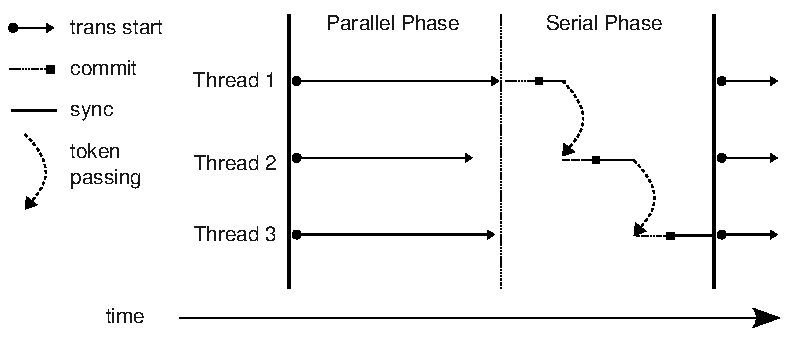
\includegraphics[width=3.25in]{fig/phase}
\caption{An overview of \dthreads{} phase. Program execution with \dthreads{} parallel and serial phases.\label{fig:phase}}
}
\end{figure}

Figure~\ref{fig:phase} illustrates the progression of parallel and serial phases. 
To guarantee determinism, \dthreads{} isolates memory accesses in parallel phase. Those memory accesses in
parallel phase can work on their private copies of different process safely, those updates won't be exposed to 
shared state in parallel phase.
When a synchronization point is reached, updates are exposed in deterministic order.  
This section describes the mechanism used to alternate between parallel and serial execution 
and guarantee deterministic commit order, and the details of commits to shared memory.

\subsubsection{Fence and Token}
% TTT: don't agree with "a global lock".
%\subsubsection{\dthreads{} Schedule}
\label{sec:schedule}

The boundary between the parallel and serial phase is the internal fence.  
It is not possible to implement the internal fence using the \texttt{pthreads} barrier 
because the number of threads required to proceed can change during execution and the \texttt{pthreads} barrier does not provide this functionality (details in Section~\ref{sec:synchronization}).

\label{sec:token}
\begin{figure}
\begin{lstlisting}
void waitFence(void) {
	lock();
	while(!isArrivalPhase()) { 
		CondWait();
	}

	waiting_threads++;
	if(waiting_threads < live_threads) {
		while(!isDeparturePhase()) {
			CondWait();
		}
	} else {
		setDeparturePhase();
		CondBroadcast();
	}

	waiting_threads--;
	if (waiting_threads == 0) {
		setArrivalPhase();
		CondBroadcast();
	}
	unlock();
}
\end{lstlisting}
\caption{Pseudocode for the internal fence.\label{fig:internalFence}}
\end{figure}

Figure~\ref{fig:internalFence} shows pseudocode for the internal fence.  Threads must wait at the fence 
until all threads from the previous 
% TTT
%parallel have departed (lines 3-5).  
%Once the fence has emptied of threads,
% Once all previous 
fence have deptarted. Those waiting threads should block until the departure phase (lines 8-11). 
% TTT_end
If the thread is the last to enter the fence, it sets the departure phase and wakes the waiting threads (lines 12-15).  
As threads leave the fence, they decrement the waiting thread count.  The last thread to leave sets the fence to the arrival phase and wakes any waiting threads (lines 17-21).

\textbf{CCC: Not edited}

\begin{figure}
\begin{lstlisting}
void waitToken() {
  waitFence();
  while(isNotMyToken()) { yield(); }
}
void putToken() {
    passTokenToNextOfTokenQueue();
}
\end{lstlisting}
\caption{Pseudocode for waitToken and putToken. waitToken() first waits at the fence (line 2) and then waits for
the token to be set to current thread (line 3).  putToken() simply
passes the token to the next thread entry in the token queue.
\label{fig:token}}
\end{figure}

Another important mechanism of \dthreads{} is the token implementation. 
In order to guarantee determinism, each thread must wait for token
before it can communicate with other threads. 
The token is one shared pointer actually, pointing to next runnable thread entry.
Since the token is unique in the whole system, it guarantees a global order for
all operations in serial phase. 

We introduce two subroutines to manage tokens. \texttt{waitToken()}
waits at the internal fence and then waits to acquire the global token
in order to enter serial mode. \texttt{putToken()} passes the token to
the next waiting thread.

To achieve determinism (see Figure~\ref{fig:phase}), those threads from parallel phase 
should wait at the internal fence before they can entering into the serial phase (actually calling
\texttt{waitToken}).
Note that it is important to wait at fence even for one thread which doomed to win the token next,
since their commits can affect other threads' behavior if no fence.
In serial phase, each thread can do those commits for parallel phase and actual synchronizations
before they passed the token to next thread. 
In the end of serial phase, we still needs to wait at fence in order to entering into next run for the same reason.


\textbf{CCC: Edited}

\subsubsection{Commit Protocol}
\begin{figure}
{\centering
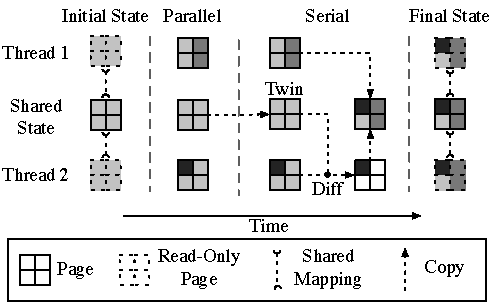
\includegraphics[width=3.25in]{fig/architecture-diagram}
\caption{An overview of \dthreads{} execution.\label{fig:architecture}}
}
\end{figure}

Figure~\ref{fig:architecture} shows the steps taken by \dthreads{} to capture modifications to shared state and expose them in a deterministic order.  At the beginning of the parallel phase, threads have a read-only mapping for all shared pages.  If a thread writes to a shared page during the parallel phase, this write is trapped and re-issued on a private copy of the shared page.  Reads go directly to shared memory and are not trapped.  In the serial phase, threads commit their updates one at a time.  The first thread to commit to a page can directly copy its private copy to the shared state, but subsequent commits must copy only the modified bytes.  This is done by diffing with the twin page, an unmodified copy of the shared page from the beginning of the serial phase.  At the end of the serial phase, private copies are released and these addresses are restored to read-only mappings of the shared memory.

\textbf{CCC: It looks like pages are write-protected in atomicBegin AND atomicEnd.  This seems redundant.}

\begin{figure}[!ht]
\begin{lstlisting}
void atomicBegin() {
	foreach(page in modifiedPages) {
		page.writeProtect();
		page.privateCopy.free();
	}
	// CCC: what does this next line do?
	cleanupDirtyPagelist(); 
}
\end{lstlisting}
\caption{Pseudocode for \texttt{atomicBegin}.\label{fig:atomicbegin}}
\end{figure}

\label{sec:atomicbegin}

Figure~\ref{fig:atomicbegin} shows pseudocode for the \texttt{atomicBegin()} function.   First, all previously-written pages are write-protected (line 3).  The old working copies of these pages are then discarded, and mappings are updated to reference the shared state (line 4).

\begin{figure}[!ht]
\begin{lstlisting}
void atomicEnd(bool doCleanup) {
	foreach(page in modifiedPages) {
		if(page.writers > 1 && !page.hasTwin()) {
			page.createTwin();
		}

		if(page.version == page.localCopy.version) {
			page.copyCommit();
		} else {
			page.diffCommit();
			// CCC: Why isn't this outside the 'if'?
			if(doCleanup) {
				page.writeProtect();
				page.privateCopy.free();
			}
		}

		page.writers = page.writers - 1;
		if(page.writers == 0 && page.hasTwin()) { 
			page.twin.free();
		}
		page.version = page.version + 1;
	}
}
\end{lstlisting}
\caption{Pseudocode for \texttt{atomicEnd}.\label{fig:atomicend}}
\end{figure}

Figure~\ref{fig:atomicend} shows the pseudocode for the \texttt{atomicend()} function.  \texttt{atomicEnd()} commits all changes from the current transaction to the shared page.  For each modified page with more than one writer, \dthreads{} ensures that a twin page is created (lines 3-5).  If the version number of the private copy matches the shared page, then this is the first thread to commit.  In this case, the entire private copy can be copied to the shared state (lines 7 and 8).  If the version numbers do not match, then another thread has already committed changes to the page and a diff-based commit must be used (lines 9-10).  If the \texttt{doCleanup} flag is set, the page is write-protected and the private copy is freed (lines 12-15).  The number of writers to the page is decremented (line 18), and if there are no writers left to commit, the twin page is freed (lines 19-21).  Finally, the shared page's version number is incremented (line 22).

\textbf{CCC: Not Edited}

\subsection{Deterministic Synchronization}
\label{sec:synchronization}

Comparing to Grace, \dthreads{} supports one complete synchronization
mechanism.  Grace turns lock operations to no-ops to eliminate
deadlocks and does not support conditional variables or barriers.  The
only supported synchronization by Grace is thread exit; Grace enforces
a sequential semantics in thread exit.

\dthreads{} supports the full range of synchronizations in the
pthreads API, including locks, conditional variables, barriers and
different kinds of thread exit.

\subsubsection{Locks}

\dthreads{} does not differentiate between specific locks by using the same global token, 
which can possibly compromise the efficiency of program. But we argue
that it is necessary to do so in order to get the complete
deterministic view of memory in the share-memory model.
Multiple locks are treated as one lock, and serial mode ends
when all locks have been unlocked. 
% EDB: We need to acquire a token before we can execute any
% synchronization operation. We only release the token once our lock
% count is 0 (for instance, lock(A); lock(B); unlock(B); unlock(A);
% we release the token only after unlock(A).


% (more reasons ******).

% critical sections are normally short, so...

\begin{figure}
\begin{lstlisting}
void mutex_lock (pthread_mutex_t * mutex) {
  if(_locks == 0) {
    waitToken();
    atomicEnd(true);
  }
  _locks++;
}
\end{lstlisting}
\begin{lstlisting}
void mutex_unlock(pthread_mutex_t * mutex) {
  _locks--;
  // Release the token when no locks are held.
  if(_locks == 0) {
    atomicEnd(false);
    putToken();
    atomicBegin();
    waitFence();
  }
}
\end{lstlisting}
\caption{Pseudocode for lock and unlock($\S$~\ref{sec:lock}).
\label{fig:lock}}
\end{figure}

\label{sec:lock}
Figure~\ref{fig:lock} presents pseudocode for \texttt{lock and unlock}.
First, it will check whether current threads has already held the token(line 2). 
If not, then current thread should wait the token in order to enter into 
the serial phase(line 3). The first thing in the serial phase is to
commit those changes of current transaction to the shared mapping and 
do some basic cleanup (line 4) (see ~\ref{sec:atomicBegic}).
In unlock(), we decrement the count for lock (line 2) and don't do anything if
lock is no equal to 0, which makes multiple locks behaving as a huge lock, potentially 
avoiding any possible deadlock problems.
If lock's count is equal to 0, we commit all memory modifications (line 5) and release
the token to next thread in the token queue (line 6). Then it can do self cleanup by calling
\texttt{atomicBegin}. After that, it simply wait at the fence in order to enter into the next
round's parallel phase (line 8).

\subsubsection{Condition Variables}

Guaranteeing determinism for condition variables is more complex than
for other synchronization operations. In this case, \dthreads{} cannot
rely on operating system support, since threads waiting on the same
condition variable can be awakened in any order. In addition, naively
imposing a global order could easily lead to deadlocks.

\label{sec:condwait}
Different with the busy wait mechanism that CoreDet used, 
\dthreads{} tries to reduce the performance cost
introduced by busy wait mechanism. Since we have no idea when those
waiting threads will be awakened, we don't want those threads to be
checked frequently since this can cause expensive process
switches. Also, we don't want those waiting threads to thwart the the
token passing of non-waiting threads.
In \dthreads{}, waiting threads are extracted from the normal run
queue and inserted into the corresponding queue of condition
variable so that the token will not be passed to these waiting
threads.

By inserting threads into corresponding queue of condition
variables, which can help those signal and broadcast function to find
out which thread should be waken up firstly and to avoid the
un-determinism brought by operating system. We enforce the
first-in-first-out rule for all waiting threads.

Since those threads calling \texttt{cond\_wait} should get the token in order
to ensure the determinism, they have to release the token to next
thread in the active list. After finishing these work, then those
threads can actuall waiting on the real process-shared conditional
variable.

After one thread is awakened, the thread should try to get token at
first in order to proceed since the thread being awakened is 
still inside the critical section (under lock protection)
and the token is required to guarantee determinism under the critical region. 

\dthreads{} uses the busy wait mechanism to get the global token. 
It is noted that this new awakened thread don't need to call waitToken() to get
token since waitToken() should wait for all alivethreads to reach the fence at first. 
Now the waking thread has already passed the fence, calling waitToken() can potentially
put this new awakened thread to the next run of serial phase, which not only hurts
the performance but also introduce some possible deadlock.

\begin{figure}
\begin{lstlisting}
void cond_wait (pthread_cond_t * cond) {
  waitToken();
  atomicEnd(false);
  removeFromTokenQueue();
  insertToTailOfCondqueue();
  decreaseInternalFence();
  putToken();
  // Only proceed if I am ready to run.
  while (!isReadyToGo()) { real_condwait(); }
  while (isNotMyToken()) { yield(); } 
  atomicBegin();
  // Token can be released in unlock. 
}
\end{lstlisting}
\caption{Pseudocode for \texttt{cond\_wait} ($\S$~\ref{sec:condwait}). 
\label{fig:condwait}}
\end{figure}

Figure~\ref{fig:condwait} presents pseudocode
for \texttt{cond\_wait}.  When a thread executes \texttt{cond\_wait},
it first awaits the token (line 2) before it can proceed.  It then
commits local modifications, removes itself from the token queue, and
places itself at the tail of conditional variable's queue (lines
3--5). It then decreases the internal fence thread count (line 6) and passes
the token to the next entry on the token queue (line 7). When a thread
is awakened by a signal, it checks whether the current thread is in
fact ready to run (line 9), since multiple threads can be awakened
by \texttt{cond\_signal} but only the first thread can run.  Finally,
it waits for the token to enter into the serial phase (line 12). 

\label{sec:condsignal}

\begin{figure}
\begin{lstlisting}
void cond_signal() {
  if(!isHoldingToken())
    waitToken();
  atomicEnd(false);
  if(noWaiters()) return;
  lock();
  thread = getFirstThreadOfCondQueue();
  insertToHeadOfTokenQueue();
  setThreadReadyToGo();
  incrementInternalFence();
  unlock();
  atomicBegin();
}
\end{lstlisting}
\caption{Pseudocode for \texttt{cond\_signal} ($\S$~\ref{sec:condsignal}). 
\label{fig:condsignal}}
\end{figure}

In \texttt{pthreads}, the only difference between \texttt{cond\_signal}
and cond\_broadcast is that \texttt{cond\_signal} only wakes up the
first thread, while cond\_broadcast wakes up all threads in the
queue. To guarantee determinism for \texttt{cond\_signal}, \dthreads{}
broadcasts the signal to all threads blocked on the condition
variable, but only the status of first thead in the queue can be set
to runnable, so other threads will have to wait on the condition
variable again (see~\ref{fig:condwait}).
These functions remove the corresponding threads from the queue
of condition variable and insert them to the header of active list,
thus those threads can get token next.  Note that it is very important
to do so both to avoid deadlock and to improve performance. By placing
awakened theads on the next runnable position rather than on the tail
of the run queue, \dthreads{} avoids possible deadlocks. 
Thus, these awakened threads can run immediately (see line 10 of Figure~\ref{fig:condwait}) 
after getting the token, which improves performance. Finally, the
signalling thread releases the token to awakened threads.

Figure~\ref{fig:condsignal} presents the pseudocode
for \texttt{cond\_signal}. Before proceeding, the caller waits for
the token if it is not holding it already, and commits any local
modifications (lines 2--4).  If there are no waiters on the
conditional variable, it returns immediately. Otherwise, \dthreads{}
removes the first thread from the condvar's queue and places it at the
head of the token queue (lines 7--8). Finally, it makes this thread
runnable and increase the internal fence's thread count (line 9--10).

\subsubsection{Barriers}

\label{sec:barrierwait}

\begin{figure}
\begin{lstlisting}
void barrier_wait() {
  waitToken(); atomicEnd(false);
 
  lock();
  if(isLastThreadEnterBarrier()) {
	moveWholelistBacktoTokenqueue();
	increaseInternalFence(waitersNumb);
	passTokenToFirstOfBarrQueue();
  } 
  else {
    removeFromTokenqueue();
	insertTailOfBarrQueue();
	putToken();
  }
  unlock();

  atomicBegin();
  realBarrierWait();  
}
\end{lstlisting}
\caption{Pseudocode for barrier\_wait ($\S$~\ref{sec:barrierwait}).
\label{fig:barrierwait}}
\end{figure}

As with condition variables, \dthreads{} must ensure that threads
waiting on a barrier do not disrupt the token passing of running
threads. \dthreads{} removes threads entering into the barrier from
the run queue and places them on the corresponding barrier queue.

To avoid blocking on the barrier, the last thread entering into
the barrier moves all threads to the runnable queue and increases
the fence's thread count.

To improve parallelization, atomicBegin() is called to write-protect 
all dirty pages and release private copies before they actually wait on 
the real process-shared barrier. Thus, the work of atomicBegin() runs in parallel
with other threads. 

Figure~\ref{fig:barrierwait} presents pseudocode
for \texttt{barrier\_wait}. The calling thread first waits for the
token to commit any local modifications in order to ensure
deterministic commit (lines 2 and 3). If the current thread is the
last to enter the barrier, then \dthreads{} moves the entire list of
threads on the barrier queue to the token queue (line 7), increases
the fence's thread count (line 8), and passes the token to the first thread in the
barrier queue (line 9).  Otherwise, \dthreads{} removes the current
thread from the token queue (line 12), places it on the barrier queue
(line 13), and releases token (line 14). Finally, the thread waits on
the actual barrier (line 19).

\subsubsection{Thread Creation and Exit}

\label{sec:threadcreation}

\begin{figure}
\begin{lstlisting}
void thread_create () {
  waitToken();
  clone(CLONE_FS| CLONE_FILES | CLONE_CHILD);
  if(isChild) {
    getGlobalThreadIndex();
	insertToTokenQueue();
	notifyChildRegistered();
	// Await notification until parent reaches 
    // next sync point after spawning.
	waitParentBroadcast();	
  }
  else if (isParent) {
	waitChildRegistered();
  }
}
\end{lstlisting}
\begin{lstlisting}
void thread_exit() {
  waitToken();
  atomicEnd(false);
  removeFromTokenQueue();
  decreaseInternalFence();
  putToken();
  exitThread(); 
}
\end{lstlisting}
\caption{Pseudocode for thread creation and exit ($\S$~\ref{sec:threadcreation}).
\label{fig:threadcreation}
}
\end{figure}

\textbf{CCC: Edited}

To guarantee determinism, thread creation and exit must be performed in the serial phase.  Newly created threads are immediately added to the token queue.  Creating a thread does not immediately release the token; this allows a single thread to quickly create multiple child threads without waiting for a new serial phase for each.

Figure~\ref{fig:threadcreation} shows pseudocode for thread creation. The caller first waits for the token before proceeding (line 2).  It then creates a new process with shared file descriptors but a distinct address space using the \texttt{clone} system call (line 3).  The newly created child obtains the global thread index (line 5), places itself in the token queue (line 6), and notifies the parent that child has registered itself in the active list (line 7). The child thread then waits for the parent to reach a synchronization point.

When \texttt{thread\_exit()} is called, the caller first waits for the token and then commits any local modifications (line 3). It then removes itself from the token queue (line 4) and decreases the number of threads required to proceed to the next phase (line 5). Finally, the thread passes its token to the next thread in the token queue (line 6) and exits (line 7).

\textbf{CCC: Not Edited}

\subsubsection{Thread Cancellation}

\dthreads{} provides the following mechanism to support
deterministic thread cancellation. First, thread cancellation can only
happen in the serial mode withholding the token, which guarantees that
only current thread trying to issue cancellation request is
running. Other threads are either waiting on condition variables or
barriers. Second, thread entry should have enough information about
their status, which can be recorded. If one thread being cancelled are
waiting on condition variable or barrier, it should be removed from
corresponding queue in order to guarantee the correctness.

\subsection{Racey Example}
% return to racey example from the top of the section, walk through an execution with dthreads

\subsection{Optimizations}
\dthreads{} does a lot of optimizations to improve the performance.

\subsubsection{Optimization for One Thread}
When only one thread is running, \dthreads{} does not provide memory protection 
and treats all synchronization operations as no-ops.

\subsubsection{Lazy Twin Creation}
Twin pages are only created when a page has multiple writers during the same transaction.  
During the commit phase, the single writer can directly copy its working copy to the shared state 
without performing a diff.  This reduces the overhead in the common case, 
where a single thread is the exclusive writer of a page.

\subsubsection{Commit Optimization}
If one thread is the only writer on one page or it is the first thread to commit a page,
they can directly copy its working copy to shared state.
We are relying on one global page version number to check that in implementation. 
In the page handler, each thread can save one version number for every dirty page. 
In the commit process, \dthreads{} could compare this local version number with global version
number to check whether this is the first writer (see Figure~\ref{fig:atomicBegin} for pseudo code).
Any other threads that have written to this page must perform a diff against the twin page.

Another optimization is to do parallization as much as possible. 
\texttt{atomicBegin} only does some laundry jobs, releasing those private page frames or resetting pages to read-only mode.
We are trying to make this to parallize with other works since it only affect one threads' behavior. 
For example, \texttt{atomicEnd} in lock operations (see Figure~\ref{fig:lock} 
not only commits, but also launders pages if
necessary. Clearly, it is safe to cleanup all dirty pages but that
brings the performance problem since it is finished in serial phase.
By using the \texttt{atomicEnd(true)}, only those pages modified by
earlier threads should be cleaned up in order to give one complete
image of one page which later transactions may refer to.


\begin{figure*}[!t]
{\centering
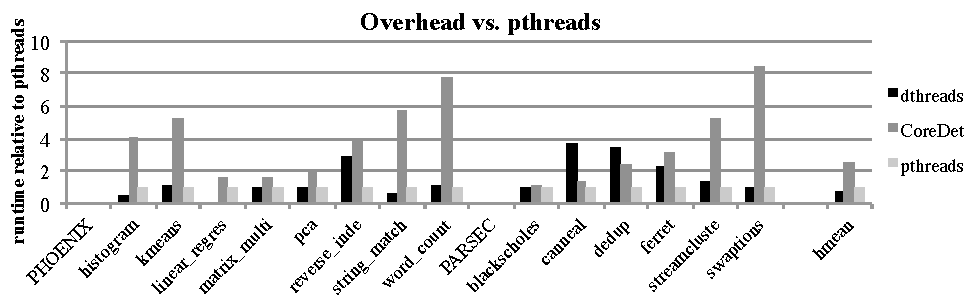
\includegraphics[width=5in]{fig/overhead-figure}
\caption{Normalized execution time with respect to \pthreads{} (lower is better). For 9 of the 14 benchmarks, \dthreads{} runs nearly as fast or faster than \pthreads{}, while providing deterministic behavior.\label{fig:performance}}
}
\end{figure*}

\section{Optimizations}
\label{sec:dthreads-optimizations}

\dthreads{} employs a number of optimizations that improve its performance.

\textbf{Lazy commit:}
\dthreads{} reduces copying overhead and the time spent in the serial
phase by \emph{lazily} committing pages. When only one thread has ever
modified a page, \dthreads{} considers that thread to be the page's
owner.  An owned page is committed to shared state only when another
thread attempts to read or write this page, or when the owning thread attempts to modify it in a later phase. \dthreads{} tracks reads with page protection and signals
the owning thread to commit pages on demand. To reduce the number of
read faults, pages holding global variables (which we expect to be
shared) and any pages in the heap that have ever had multiple writers are
all considered unowned and are not read-protected.

\textbf{Lazy twin creation and diff elimination: }
To further reduce copying and memory overhead, a twin page is only created
when a page has multiple writers during the same transaction.
In the commit phase, a single writer can directly copy its working copy to
shared state without performing a diff. \dthreads{} does this by
comparing the local version number to the global page version number
for each dirtied page.  At commit time, \dthreads{} directly copies
its working copy for each page whenever its local version number
equals its global version number.  This optimization saves the cost of a twin 
page allocation, a page copy, and a diff in the common case where just one thread is the sole writer of a page.

\textbf{Single-threaded execution: }
Whenever only one thread is running, \dthreads{} stops using memory protection 
and treats certain synchronization operations (locks and barriers) as no-ops.
In addition, when all other threads are waiting on condition variables, 
\dthreads{} does not commit local changes to the shared mapping or discard  
private dirty pages. Updates are only committed when the thread
issues a signal or broadcast call, which wakes up at least one thread
and thus requires that all updates be committed.

\textbf{Lock ownership: }
\dthreads{} uses lock ownership to avoid unnecessary waiting when threads are
using distinct locks.  Initially, all locks are unowned.  Any thread that
attempts to acquire a lock that it does not own must wait until the serial phase
to do so.  If multiple threads attempt to acquire the same lock, this lock is 
marked as shared.  If only one thread attempts to acquire the lock, this thread 
takes ownership of the lock and can acquire and release it during the parallel
phase.

Lock ownership can result in starvation if one thread continues to re-acquire an owned lock without entering the serial phase.  To avoid this, each lock has a maximum number of times it can be acquired during a parallel phase before a serial phase is required.

\textbf{Parallelization: }
\dthreads{} attempts to expose as much parallelism as possible in the
runtime system itself.  One optimization takes place at the start of trasactions, where
\dthreads{} performs a variety of cleanup tasks. These include releasing private page frames,
and resetting pages to read-only mode by calling the \texttt{madvise}
and \texttt{mprotect} system calls. If all this cleanup work is done
simultaneously for all threads in the beginning of parallel phase
(Figure~\ref{fig:phase}), this can hurt performance for some
benchmarks.

Since these operations do not affect other the behavior of other
threads, most of this work can be parallelized with other threads'
commit operations without holding the global token. With this
optimization, the token is passed to the next thread as soon as
possible, saving time in the serial phase.  Before passing the token,
any local copies of pages that have been modified by other threads
must be discarded, and the shared read-only mapping is restored.  This
ensures all threads have a complete image of this page which later
transactions may refer to.  In the actual
implementation, this cleanup occurs at the end of each transaction.



\section{Evaluation}
\label{sec:evaluation}

% CCC: overhead figure moved to main.tex to place on the same page as evaluation section

\begin{figure*}
{\centering
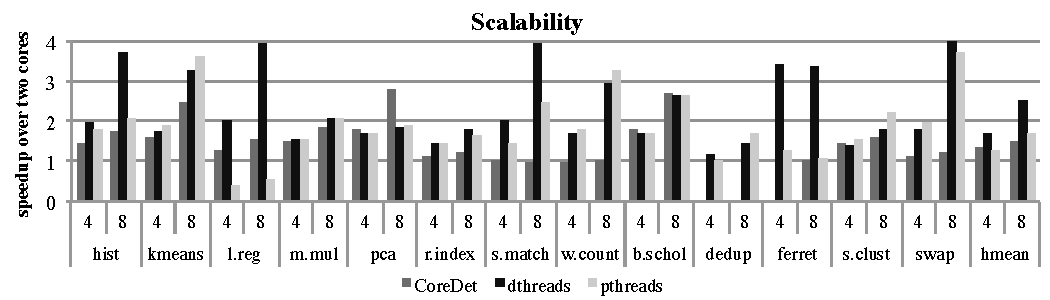
\includegraphics[width=5in]{fig/scalability-figure}
\caption{
	Speedup with four and eight cores relative to two cores (higher is better).  \dthreads{} generally scales nearly as well or better than \pthreads{} and almost always as well or better than CoreDet.  CoreDet was unable to run \texttt{dedup} with two cores and \texttt{ferret} with four cores, so some scalability numbers are missing.\label{fig:scalability}}
}
\end{figure*}
\begin{figure*}[htb]
{\centering
\tiny
\subfigure{\lstinputlisting[numbers=none,frame=none,boxpos=t]{predator/figure/linearregression.report}}
\caption{An example report by \Predator{} indicating false sharing in the linear\_regression benchmark.
\label{fig:lrreport}}
}
\end{figure*}



\label{sec:evaluation}

This section answers the following questions:
\begin{itemize}
\item
  How effective is \Predator{} at detecting and predicting false sharing?

\item
  What is \Predator{}'s overhead, in terms of execution time and memory ?

\item
  How sensitive is \Predator{} to different sampling rates?
 
\end{itemize}

\paragraph{Experimental Platform.} All evaluations are performed on a quiescent Intel Core 2 dual-processor system equipped with 
16GB RAM. Each processor is a 4-core 64-bit Intel Xeon running at 2.33 GHz, with a 4MB shared L2 cache and 32KB private L1 cache. The underlying operating system is an unmodified CentOS 5.5, running with Linux kernel version 2.6.18-194.17.1.el5. The glibc version is 2.5. 

\paragraph{Evaluated Applications.}
This paper evaluates two popular benchmark suites,
Phoenix (with large input) ~\cite{phoenix-hpca} and PARSEC (with simlarge input) ~\cite{parsec}. Even with unmodified LLVM-3.2, Facesim cannot be compiled successfully (having complaints on an undefined template) and Canneal aborts unexpectedly. Thus, these two benchmarks are excluded.
We also evaluate \Predator{} on six real applications, including MySQL, Boost, Memcached, aget, pbzip2 and pfscan.



\subsection{Detection and Prediction Effectiveness}
\label{sec:effective}

For every false sharing problem, \Predator{} reports source code information and detailed memory access information in order to help users fix those problems. Figure~\ref{fig:lrreport} shows an example for the linear\_regression benchmark. This report shows that the heap object starting with $0x40000038$ potentially causes a large number of cache invalidations. The call stack of allocation is provided to help locate culprits. In addition, \Predator{} also reports word-level access information of this object, which helps to identify where and how false sharing occurs. From that, we can know that it is a latent false sharing problem predicted by \Predator{}, since different threads are accessing different cache lines. 

\subsubsection{Benchmarks}
\label{sec:benchmarks}

\begin{table*}[!t]
{\centering\begin{tabular}{l|r|r|r|r|r}\hline
{\bf \small Benchmark} & {\bf \small Source Code} & {\bf \small New} & {\bf \small Without Prediction} &{\bf \small With Prediction} & {\bf \small Improvement} \\
\hline
\small \textbf{histogram} & {\small histogram-pthread.c:213} & \cmark{} &\cmark{} & \cmark{} & 46.22\%\\
\small \textbf{linear\_regression} & {\small linear\_regression-pthread.c:133} & & & \cmark{} & 1206.93\% \\
\small \textbf{reverse\_index} & {\small reverseindex-pthread.c:511} & & \cmark{} & \cmark{} & 0.09\%\\
\small \textbf{word\_count} & {\small word\_count-pthread.c:136} & & \cmark{} & \cmark{} & 0.14\%\\
\hline
\small \textbf{streamcluster} & {\small streamcluster.cpp:985} &  & \cmark{} & \cmark{} &7.52\% \\
\small \textbf{streamcluster} & {\small streamcluster.cpp:1907} & \cmark{} & \cmark{} & \cmark{} & 4.77\%\\
\hline
\end{tabular}
\caption{False sharing problems in the Phoenix and PARSEC benchmark suites. \label{table:detection}}
}
\end{table*}

Table~\ref{table:detection} provides detection results of two benchmark suites, Phoenix and PARSEC
The first column lists those programs with false sharing problems.  The second column shows precisely where the problem is. Because all discovered false sharing occurs inside heap objects, we show callsite source code information here.  The third column, ``New'', marks whether this false sharing was newly discovered by \Predator{}.  A checkmark in the following two columns indicates whether the false sharing was identified without
prediction and/or with prediction.  The final column, ``Improvement'', shows the performance improvement after fixing false sharing.
%The number is based on the average runtime of $10$ runs. 

As shown in the table, \Predator{} reveals two unknown false sharing problems. It is the first tool to detect the false sharing problems in histogram and in line $1908$ of streamcluster. 
In histogram, multiple threads simultaneously modify different locations of the same heap object, thread\_arg\_t. 
Padding this data structure fixes the false sharing problem and improves the performance by around 46\%. In streamcluster, multiple threads are simultaneously accessing and updating the same \texttt{bool} array, switch\_membership. Simply changing all elements of this array to a long type reduces the false sharing and improves the performance by about 4.7\%.

%, although it is not a complete fix of false sharing. 
%None of these two false sharing problems has been reported by previous tools.
Other false sharing problems were discovered by previous work~\cite{sheriff}. We do not see significant performance improvement for reverse\_index and word\_count benchmarks. They are reported here because the number of cache invalidations in these two programs reaches our predefined threshold.
Making the reporting threshold higher can avoid the report of those insignificant false sharing problems.
It is worth noting that these two benchmarks definitely have false sharing problems,
which can be confirmed by word-level information generated by \Predator{}. 

The streamcluster benchmark has another false sharing problem at line $985$. Different threads change the work\_mem object simultaneously. Authors of streamclsuter have already realized this problem and provide a CACHE\_LINE macro. Unfortunately, the default value of this macro is set to $32$ bytes, which is different from the actual cache line size of the experimental machine. By setting it to $64$ bytes instead, it achieves  performance improvement of about 7.5\%.

linear\_regression has a severe false sharing problem. Fixing it improves the performance by more than $12\times$. In this benchmark, different threads update their thread-specific locations inside the tid\_args object in a tight loop. According to the observation of Nanavati et al., this false sharing problem occurs when using clang and disappears when using gcc with the -O2 and -O3 optimization level~\cite{OSdetection}. But we observed a different result when using the clang-3.2 compiler and our custom memory allocator: the false sharing problem does not occur at all because the offset of the starting address of the potentially falsely-shared object and the start of cache line is 56 bytes (see Figure~\ref{fig:perfsensitive}). With prediction mechanism, \Predator{} detects this latent false sharing problem, exemplifying the necessity of a predictive detection tool. 

\subsubsection{Real Applications}
To verify \Predator{}'s practicality, we further evaluate several widely-used real applications, whereas no previous work has done this. These real applications include a server application (MySQL~\cite{mysql}),
a standard C++ library (Boost~\cite{libfalsesharing}),
a distributed memory object caching system (Memcached), a network retriever (aget),
a parallel bzip2 file compressor (pbzip2), and a parallel file scanner (pfscan).

MySQL-5.5.32 and boost-1.49.0 are known to have false sharing problems. Other applications (memcached-1.4.15, aget-0.4.1 and pbzip2-1.1.6) do not have known false sharing problems.

The false sharing of MySQL has caused a significant scalability problem and was very difficult to identify.
According to the architect of MySQL, Mikael Ronstrom, ``we had gathered specialists on InnoDB..., participants from MySQL support... and a number of generic specialists on 
computer performance...'', ``[we] were able to improve MySQL performance by 6$\times$ with those scalability fixes''~\cite{mysql}. 
The false sharing inside Boost is caused by the usage of a  spinlock pool. Different threads may utilize different spinlocks located in the same cache line in this case. Fixing it brings a 40\% performance improvement.
\Predator{} is able to pinpoint false sharing locations in both MySQL and the Boost library. 
For the other four applications, \Predator{} does not find severe false sharing problems.

\subsubsection{Prediction Effectiveness}
\label{sec:predicteval}
In this section, we verify whether prediction can always  reveal un-observed false sharing problems.

The linear\_regression benchmark is selected here because of the following two reasons: (1) The false sharing problem of this benchmark cannot be detected without prediction; (2) False sharing severely degrades performance when it actually occurs. Hence, it is a serious problem that should always be detected. 

\begin{figure}[!t]
{\centering
\subfigure{\lstinputlisting[numbers=none,frame=none,boxpos=t]{predator/figure/linearregression.psedocode}}
\caption{The false sharing problem inside the linear\_regression benchmark: multiple threads simultaneously update their entries in lreg\_args.
\label{fig:linearregression}}
}
\end{figure}

Figure~\ref{fig:linearregression} shows the data structure and the source code exercising appropriate false sharing. The size of this data structure, lreg\_args, is $64$ bytes 
when the program is compiled to a $64$-bit binary. For this benchmark, the main thread allocates an array, containing as many elements as the number of underlying hardware cores. Each element is a lreg\_args type with $64$ bytes. This array is then passed to different threads (lreg\_thread function) so that each thread only updates its thread-dependent area. False sharing occurs if two threads happen to update data in the same cache line. 

Figure~\ref{fig:perfsensitive} shows how sensitive the performance is to different starting addresses of a falsely-shared object. When the offset is $0$ or $56$ bytes, this benchmark achieves its optimal performance and has no false sharing. When the offset is $24$ bytes, the benchmark runs around $15$ times slower than its optimal performance because of the false sharing problem.

Our evaluation shows that \Predator{} can always detect the false sharing problem with prediction enabled, demonstrating its effectiveness.

\subsection{Performance Overhead}
\label{sec:perfoverhead}

\begin{figure*}[!t]
\centering
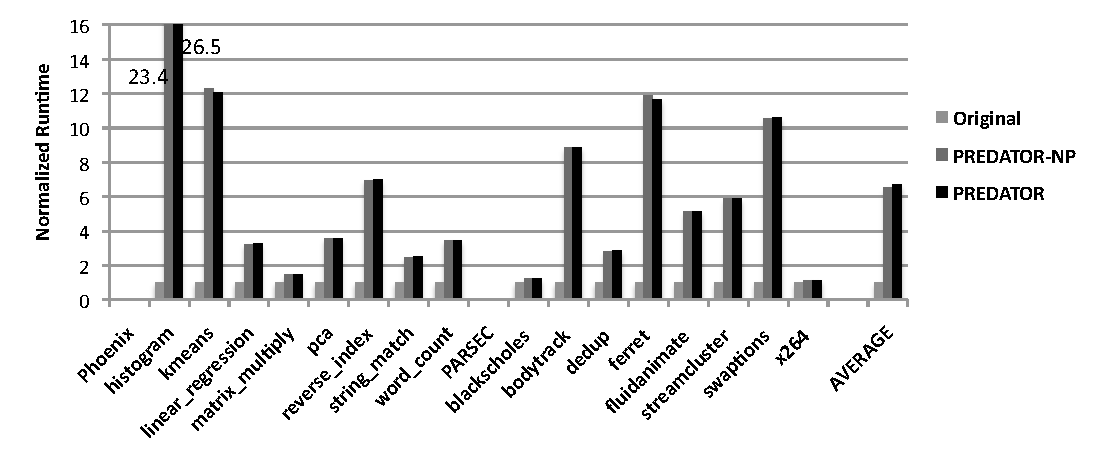
\includegraphics[width=6in]{predator/figure/perf}
\caption{
Performance overhead of \Predator{} with and without prediction(PREDATOR-NP).
\label{fig:perf}}
\end{figure*}

To avoid the effect caused by extreme outliers, all performance data shown in Figure~\ref{fig:perf} is based on the average of $10$ runs, excluding the maximum and minimum values. 

For $16$ benchmarks from the Phoenix and PARSEC benchmark suites and six real applications, \Predator{} imposes $5.4\times$ performance overhead. There is no noticeable difference on performance whether the prediction mechanism is enabled or not. 
 
Among these programs, five of them, histogram, kmeans, bodytrack, ferret, and swaptions, have more than $8\times$ performance overhead. The histogram benchmark runs more than $26\times$ slower than original executions with \pthreads{} library, because tracking detailed access on cache lines with false sharing exacerbates the false sharing effect (see more discussion in Section~\ref{sec:sample}).  For bodytrack and ferret, although there is no false sharing, \Predator{} detects a large amount of cache lines with writes larger than {\it Tracking-Threshold}. Thus, tracking those accessing details for those cache lines imposes significant performance overhead. Currently, we cannot identify the reasons why kmeans runs very slowly on \Predator{}.
   
\Predator{} imposes a small performance overhead for IO-bound applications, such as matrix\_multiply, blackscholes, x264, aget, Memcached, pbzip2, and pfscan, since \Predator{} does not add any performance overhead for IO operations.  

\subsection{Memory Overhead}
\label{sec:memoverhead}
We only evaluate the physical memory overhead of \Predator{}, instead of the virtual memory overhead, because \Predator{} allocates four gigabytes virtual memory for its custom memory allocator. Proportional set size (PSS) in \texttt{/proc/self/smaps} reflects the physical memory increase on the existing system of running an application~\cite{memusage}. Thus, we periodically collect this data and use the sum of different memory mappings as the total physical memory usage of running an application. We present the maximum value of physical memory usage in Figure~\ref{fig:memusage}. 

\Predator{} imposes less than 50\% memory overhead for 17 out of 22 applications.  For swaptions and aget, \Predator{} introduces more memory overhead because the original memory footprints of them are very small, only $3$ kilobytes. Adding the code of detection, prediction and reporting contributes to a large ratio of memory overhead. We are not clear why MySQL consumes much more memory than others. Although the average memory usage of all applications is over $2\times$, the total memory usage overhead is only about $40\%$ on \Predator{}. 


\subsection{Sensitivity to Different Sampling Rates}
\label{sec:sensitivity}
In Section~\ref{sec:sample}, we discuss that \Predator{} utilizes the sampling mechanism to reduce the tracking overhead. Running an application with different sampling rates does not affect its memory usage. Thus, we only evaluate the effect of different sampling rates on performance and effectiveness. 

The default sampling rate used by \Predator{} is 1\%. In this section, we also evaluate two other sampling rates, 0.1\% and 10\%. The performance results under the three different sample rates are shown in Figure~\ref{predator/figure:sample}. \Predator{} introduces less performance overhead under a lower sampling rate, which meets our expectation. Concerning effectiveness, even using the 0.1\% sampling rate, \Predator{} can still detect all false sharing problems, but with a lower number of cache invalidations. Thus, different sampling rates do not affect the detection effectiveness.
 
\begin{figure*}[!t]
\centering
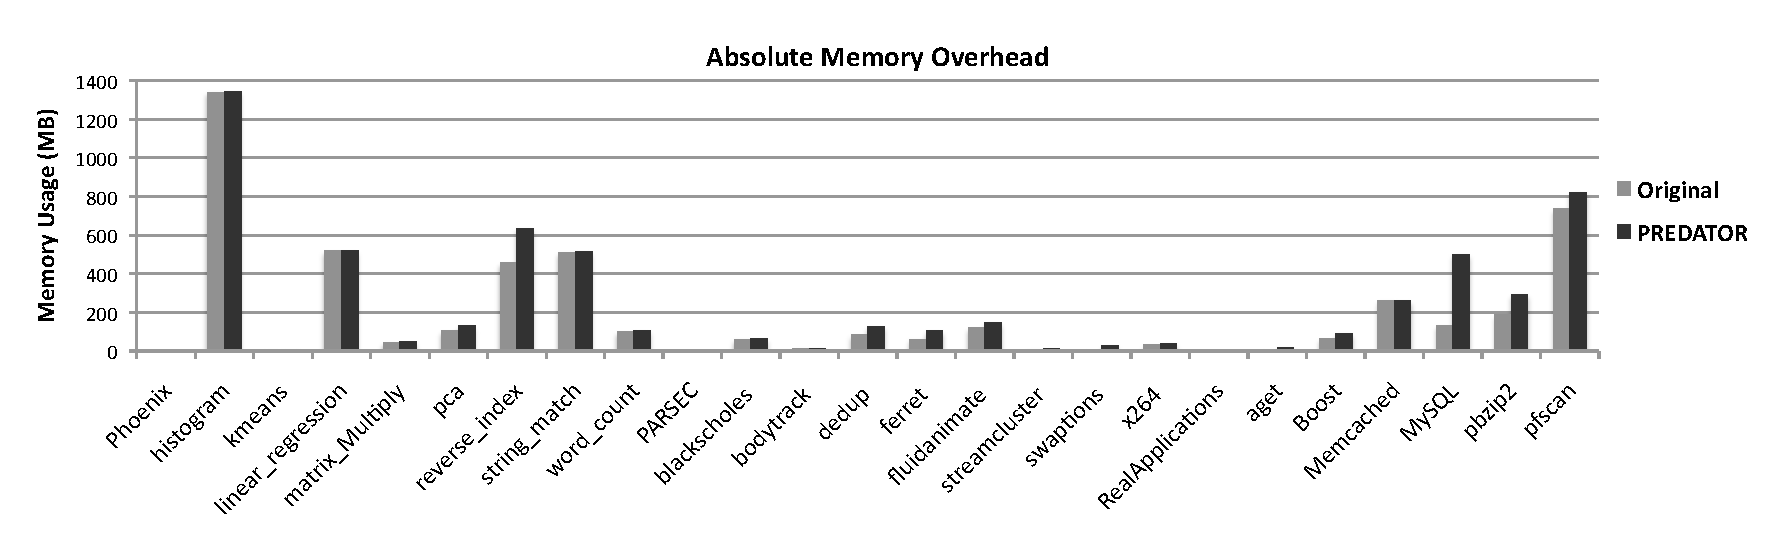
\includegraphics[width=6in]{predator/figure/absolutememory}
\caption{Absolute physical memory usage overhead with \Predator{}.}
\label{fig:absolutememusage}
\end{figure*}

\begin{figure*}[!t]
\centering
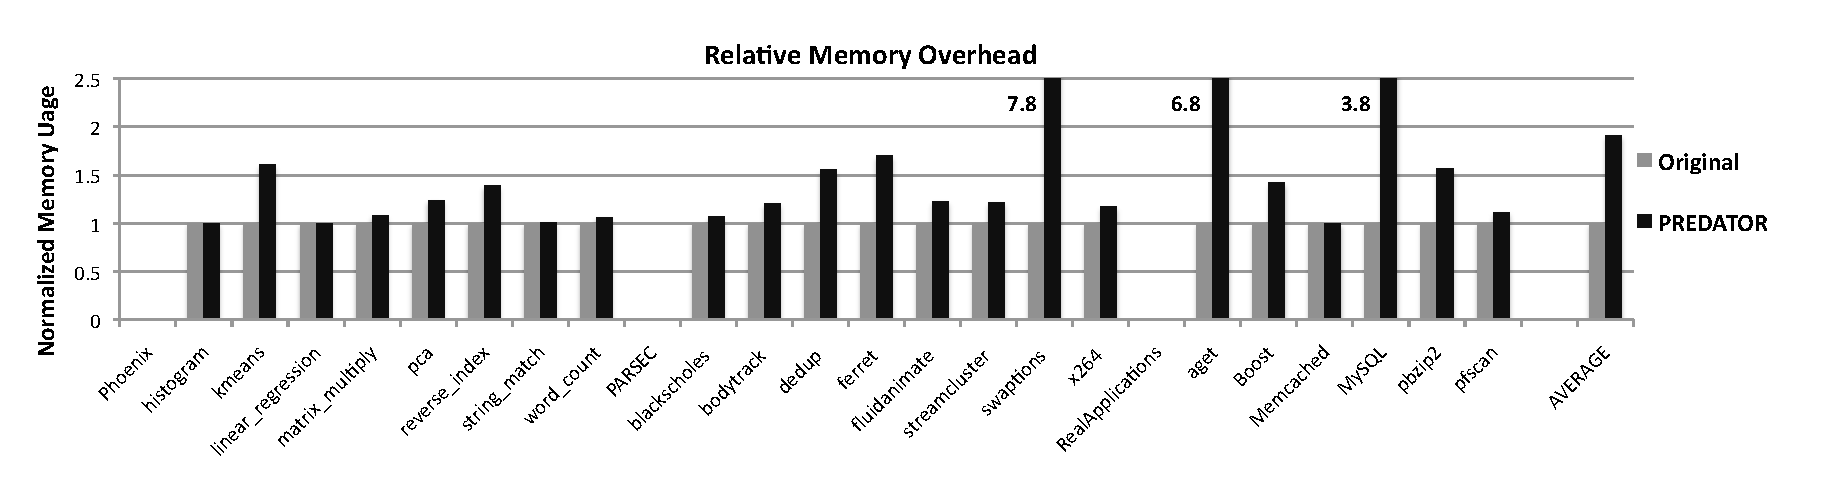
\includegraphics[width=6in]{predator/figure/memusage}
\caption{Relative physical memory usage overhead with \Predator{}.}
\label{fig:memusage}
\end{figure*}



\section{Discussion}
\label{sec:discussion}

This section analyzes some key limitations of \dthreads{} that
restrict its ability to run certain programs, limit the extent of
determinism it can guarantee, or potentially affect performance.


\textbf{Unsupported programs: }
\dthreads{} currently does not support programs with ad hoc
synchronizations, such as those that use atomic operations implemented in assembly.  However, the upcoming C++0X standard includes a library interface for atomic operations~\cite[pp. 1107--1128]{c++0xstandarddraft}, and a future version of \dthreads{} could correctly implement these by intercepting
these library calls and treating them as synchronization points. While
ad hoc synchronization is a common practice, it is also a notorious
source of bugs; Xiong et al.\ show that 22--67\% of the uses of ad hoc
synchronization lead to bugs or severe performance issues~\cite{ad-hoc-considered-harmful}.

\dthreads{} also currently does not write-share the stack
across threads, so that updates made by a thread to a stack variable
would not be reflected back to the parent, which could cause a program
to fail. Passing stack variables to a thread for modification is
extremely error-prone and generally deprecated, making this a rare
coding practice.

\textbf{External determinism: }
While \dthreads{} provides internal determinism, it does not
guarantee determinism when a program's behavior depends on external
sources of non-determinism, such as system time or I/O
events. Incorporation of \dthreads{} in the dOS framework, an OS
proposal that enforces system-level determinism, would provide full
deterministic execution, although this remains future
work~\cite{deterministic-process-groups}.

\textbf{Runtime performance: }
Section~\ref{sec:evaluation} shows that \dthreads{} can provide high
performance for a number of applications; in fact, for the majority of
the benchmarks examined, \dthreads{} matches or even exceeds the
performance of \pthreads{}. However, \dthreads{} could occasionally
degrade performance, sometimes substantially. One way it could do so
would be to exhibit an intensive use of locks (that is, acquiring and
releasing locks at high frequency), which are much more expensive
in \dthreads{} than in \pthreads{}. However, because of its determinism guarantees, \dthreads{} could allow programmers to greatly reduce their use of locks, and thus improve performance. Other application characteristics, also explored in Section~\ref{sec:performance}, can also impair performance
with \dthreads{}.


%  Since Surprise locking inside libraries. Not a limitation \emph{per
%  se} but definitely an issue that could surprise programmers.

% Draft can be downloaded from http://www.open-std.org/jtc1/sc22/wg21/docs/papers/2010/n3126.pdf.
%Fine once they are library calls, as they are in gcc and in the upcoming C++0X standard (cite!), since then we can intercept them.

\textbf{Memory consumption: }
Finally, because \dthreads{} creates private, per-process copies of
modified pages between commits, it can increase a program's memory
footprint by the number of modified pages between synchronization
points. This increased footprint does not seem to be a problem in
practice, both because the number of modified pages is generally far
smaller than the number of pages read, and because it is transitory:
all private pages are relinquished to the operating system
(via \texttt{madvise()}) at the end of every commit operation.

%Increased memory footprint (linear in the number of dirtied (modified) pages).




\punt{
\section{Future Work}
\label{sec:future-work}

Currently, we haven't handle those external non-determinism, for example, network input or timing,
which can affect the determinism if the applications are relying on that. 
One part of our future work wants to support these external non-determinism by using a shim layer to record those
external non-deterministic events. 
%Also, in current version, those memory allocation can be non-deterministic, which can potentially introduce some non-determinism if one application includes some un-safe memory operations. So we can easily to avoid this problem
%by recording those order to allocate one superblock.

Another part of our future-work are trying to handle the performance problem brought by too many dirty pages.
We can keep track of the ownership of one memory page. If one memory page is owned by one thread, normally
we don't need to commit those changes to the shared mapping. So page commits can be limitted to 
those actually shared page, hopefully we can improve the performance by using this mechanism.

%Replace effective single lock with guaranteed ordering on locks.
%Adopt ownership protocol a la DMP-O?
%Improve the determinism brought by the memory allocation, then we can fix those problem caused by un-safe memory operations.
%Support for external non-determinism.

% eliminate global lock
% possibly adopting a page-ownership protocol as used by ...
}

\section{Conclusion}
\label{sec:conclusion}

\dthreads{} is a deterministic replacement for the \pthreads{}
library that supports general-purpose multithreaded
applications. \dthreads{} is straightforward to deploy, requiring no
source code, and operates on commodity hardware. By converting threads
into processes, \dthreads{} leverages process isolation and virtual
memory protection to track and isolate concurrent memory updates with
low overhead. By committing these changes deterministically at natural
synchronization points in the code, rather than at boundaries based on
hardware performance counters, \dthreads{} not only ensures full
internal determinism---eliminating data races as well as
deadlocks---but does so in a way that is portable and easy to
understand. Its software architecture prevents false sharing, a
notorious performance problem for multithreaded applications running
on multiple, cache-coherent processors. The combination of these
approaches enables \dthreads{} to match or even exceed the performance
of \pthreads{} for the majority of the benchmarks examined here,
making \dthreads{} a safe and efficient alternative to \pthreads{} for
some applications.


\section{Acknowledgements}
The authors thank Robert Grimm, Sam Guyer, Shan Lu, Tom Bergan, Daan
Leijen, Dan Grossman, Yannis Smaragdakis, the anonymous reviewers, and our
shepherd Steven Hand for their invaluable feedback and suggestions which helped
improve this paper. We acknowledge the support of the Gigascale
Systems Research Center, one of six research centers funded under the
Focus Center Research Program (FCRP), a Semiconductor Research
Corporation entity.  This material is based upon work supported by
Intel, Microsoft Research, and the National Science Foundation under
CCF-1012195 and CCF-0910883. Any opinions, findings, and conclusions
or recommendations expressed in this material are those of the
author(s) and do not necessarily reflect the views of the National
Science Foundation.

{
\bibliographystyle{abbrv}
\bibliography{dthreads,emery}
}

\end{document}
